\chapter{Introduction}
\label{chapterlabel1}

\section{Project context and justification}

\textit{What is OSM and why is it useful in a humanitarian context? Why is data maintenance an important topic to consider with respect to humanitarian mapping? How will the outcomes of this work be relevant and useful?}

\section{Scope of work}

\textit{Outline case study approach. This is an initial exploratory study. We will be offering recommendations, but will not be making broad generalizations aout phenomena.}

\section{Research question and objectives}

\textit{How can we identify data maintenance following humanitarian mapping, and what factors relating to the dynamics of data production are related to greater data maintenance?}

\section{Research outline}

\textit{Signposting paragraphs to broadly outline each of the chapters. What will be discussed in each chapter?}

\section{Sample formatting}

% https://texblog.org/2017/02/06/proper-tables-with-latex/
\begin{table}[ht]
\centering
\caption{This is an example table}
\begin{tabular}[t]{lcc}
\toprule
Test&Treatment A&Treatment B\\
\midrule
John Smith&1&2\\
Jane Doe&--&3\\
Mary Johnson&4&5\\
\bottomrule
\end{tabular}
\end{table}%

\begin{table}[ht]
\centering
\caption{This is another example table}
\begin{tabular}[t]{lcc}
\toprule
Test&Treatment A&Treatment B\\
\midrule
John Smith&1&2\\
Jane Doe&--&3\\
Mary Johnson&4&5\\
\bottomrule
\end{tabular}
\end{table}%

\begin{figure} [H] % opens the figure environment. the '[H]' forces the image to be Here
    \centering % puts the image in the horizontal centre of the page
    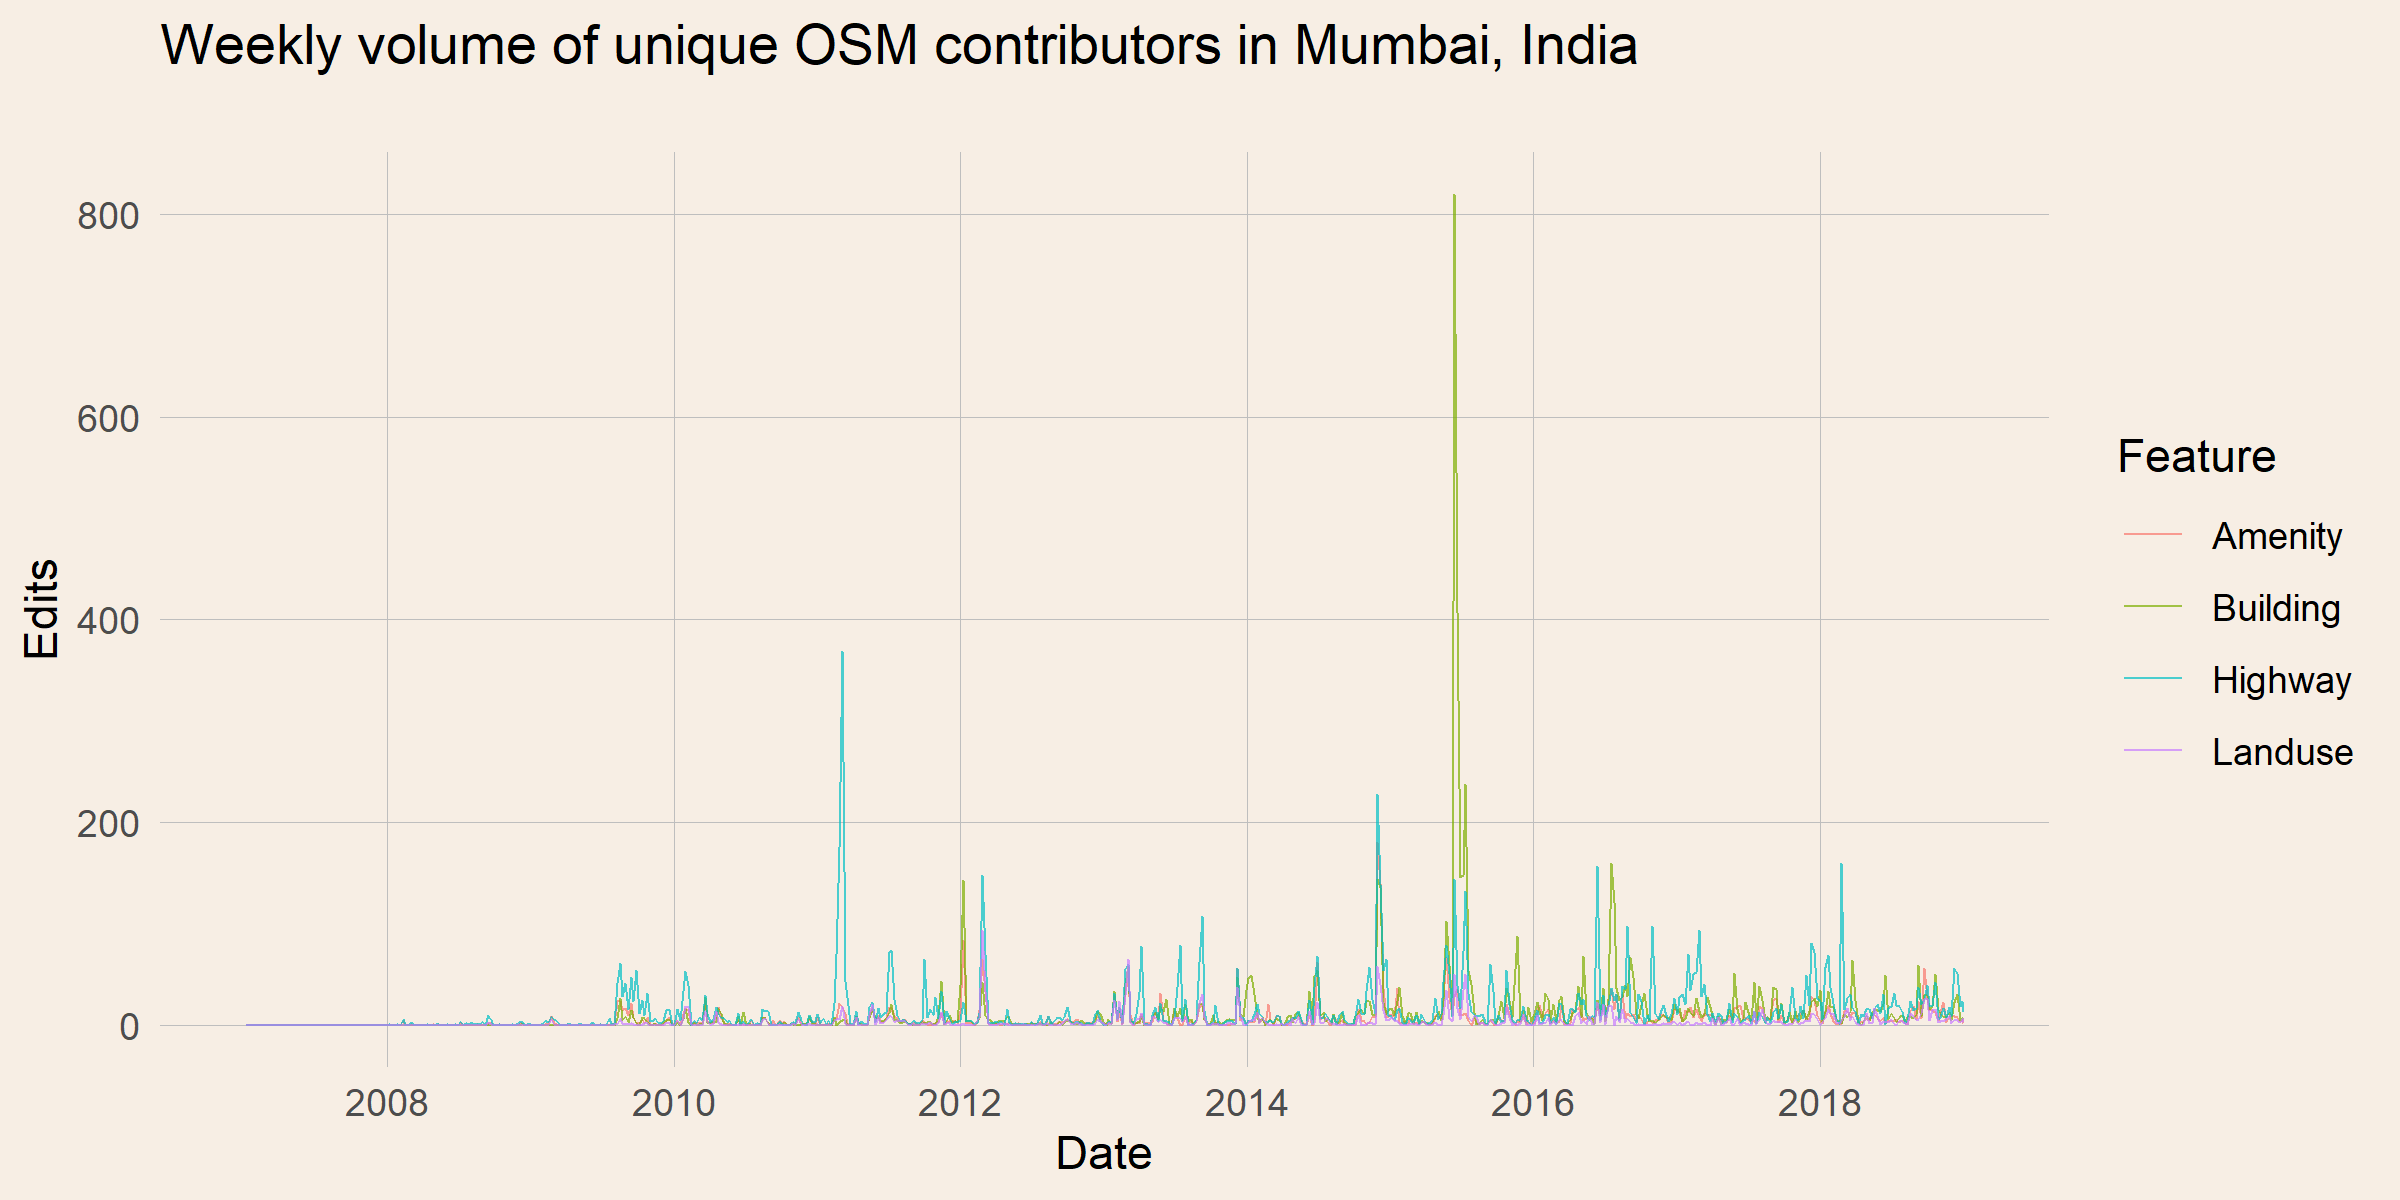
\includegraphics[width = \textwidth]{Images/mb_users_agg.png} %this tells latex what graphics to include. I put my images in an 'Images' folder to aid file management, hence the Images/ before the file name. the width bit before allows you to alter the width of the image. It is also possible to use scale as well as using equations with the textwidth to make it say half the text width.
    \caption{This is an example image} % this prints the caption below the figure
    \label{fig:four} % this internally labels the figure for future referencing.
\end{figure}

\textbf{this is bold text} and \textit{this is italicized text}. ctrl b and ctrl i work as shortcuts. 

Create an ordered list 

\begin{enumerate}
    \item Enumerate
    \item lists
    \item look
    \item like
    \item this.
\end{enumerate}

Create an unordered list 

\begin{itemize}
    \item Itemize
    \item lists
    \item look
    \item like
    \item this.
\end{itemize}

Create a nested list 

\begin{enumerate}
    \item Wow
    \begin{enumerate}
        \item another
        \begin{enumerate}
            \item nested
            \begin{enumerate}
                \item list
            \end{enumerate}
        \end{enumerate}
    \end{enumerate}
\end{enumerate}